\subsection{Empirical Questions \points{10}}

The following questions should be completed after you work through the programming portion of this assignment (Section \ref{sec:code}). 

\begin{enumerate}
\item \textbf{[4 points]} Run Q-learning on the mountain car environment using both tile and raw features. 

For the raw features: run for 2000 episodes with max iterations of 200, $\epsilon$ set to 0.05, $\gamma$ set to 0.999, and a learning rate of 0.001. 

For the tile features: run for 400 episodes with max iterations of 200, $\epsilon$ set to 0.05, $\gamma$ set to 0.99, and a learning rate of 0.00005.

For each set of features, plot the return (sum of all rewards in an episode) per episode on a line graph. On the same graph, also plot the rolling mean over a 25 episode window. Comment on the difference between the plots.

\begin{tcolorbox}[fit,height=12cm, width=\linewidth, blank, borderline={1pt}{-2pt},nobeforeafter]
%solution
\end{tcolorbox}

\end{enumerate}

\begin{figure}[H]
    \centering
    \begin{subfigure}{0.5\textwidth}
        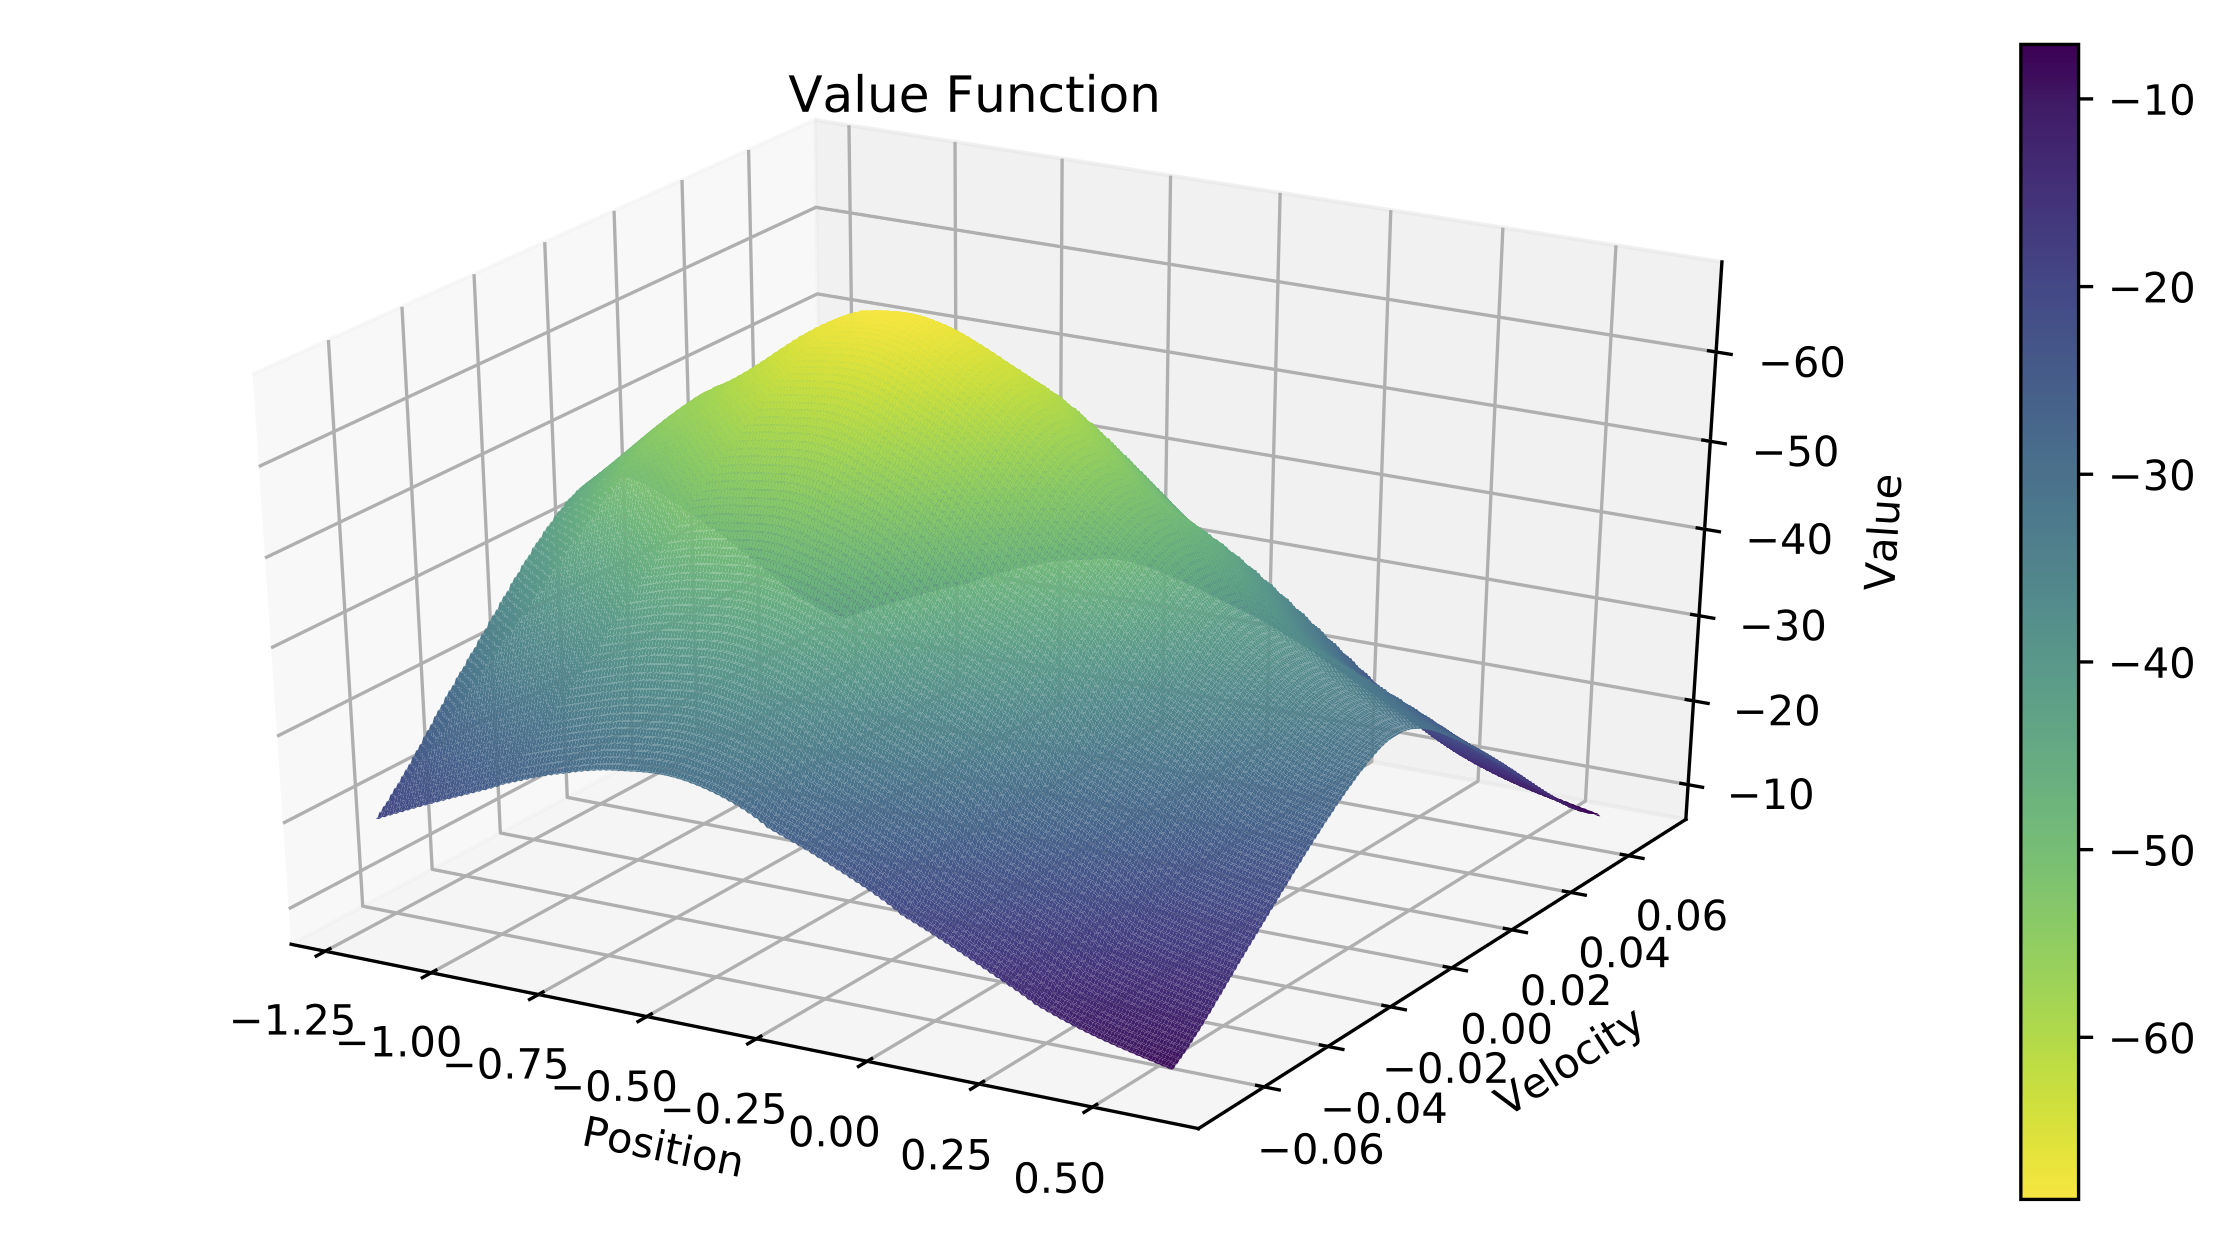
\includegraphics[width=\linewidth]{figs/value_A.png}
        \caption{}
        \label{fig:value_a}
    \end{subfigure}%
    \begin{subfigure}{0.5\textwidth}
        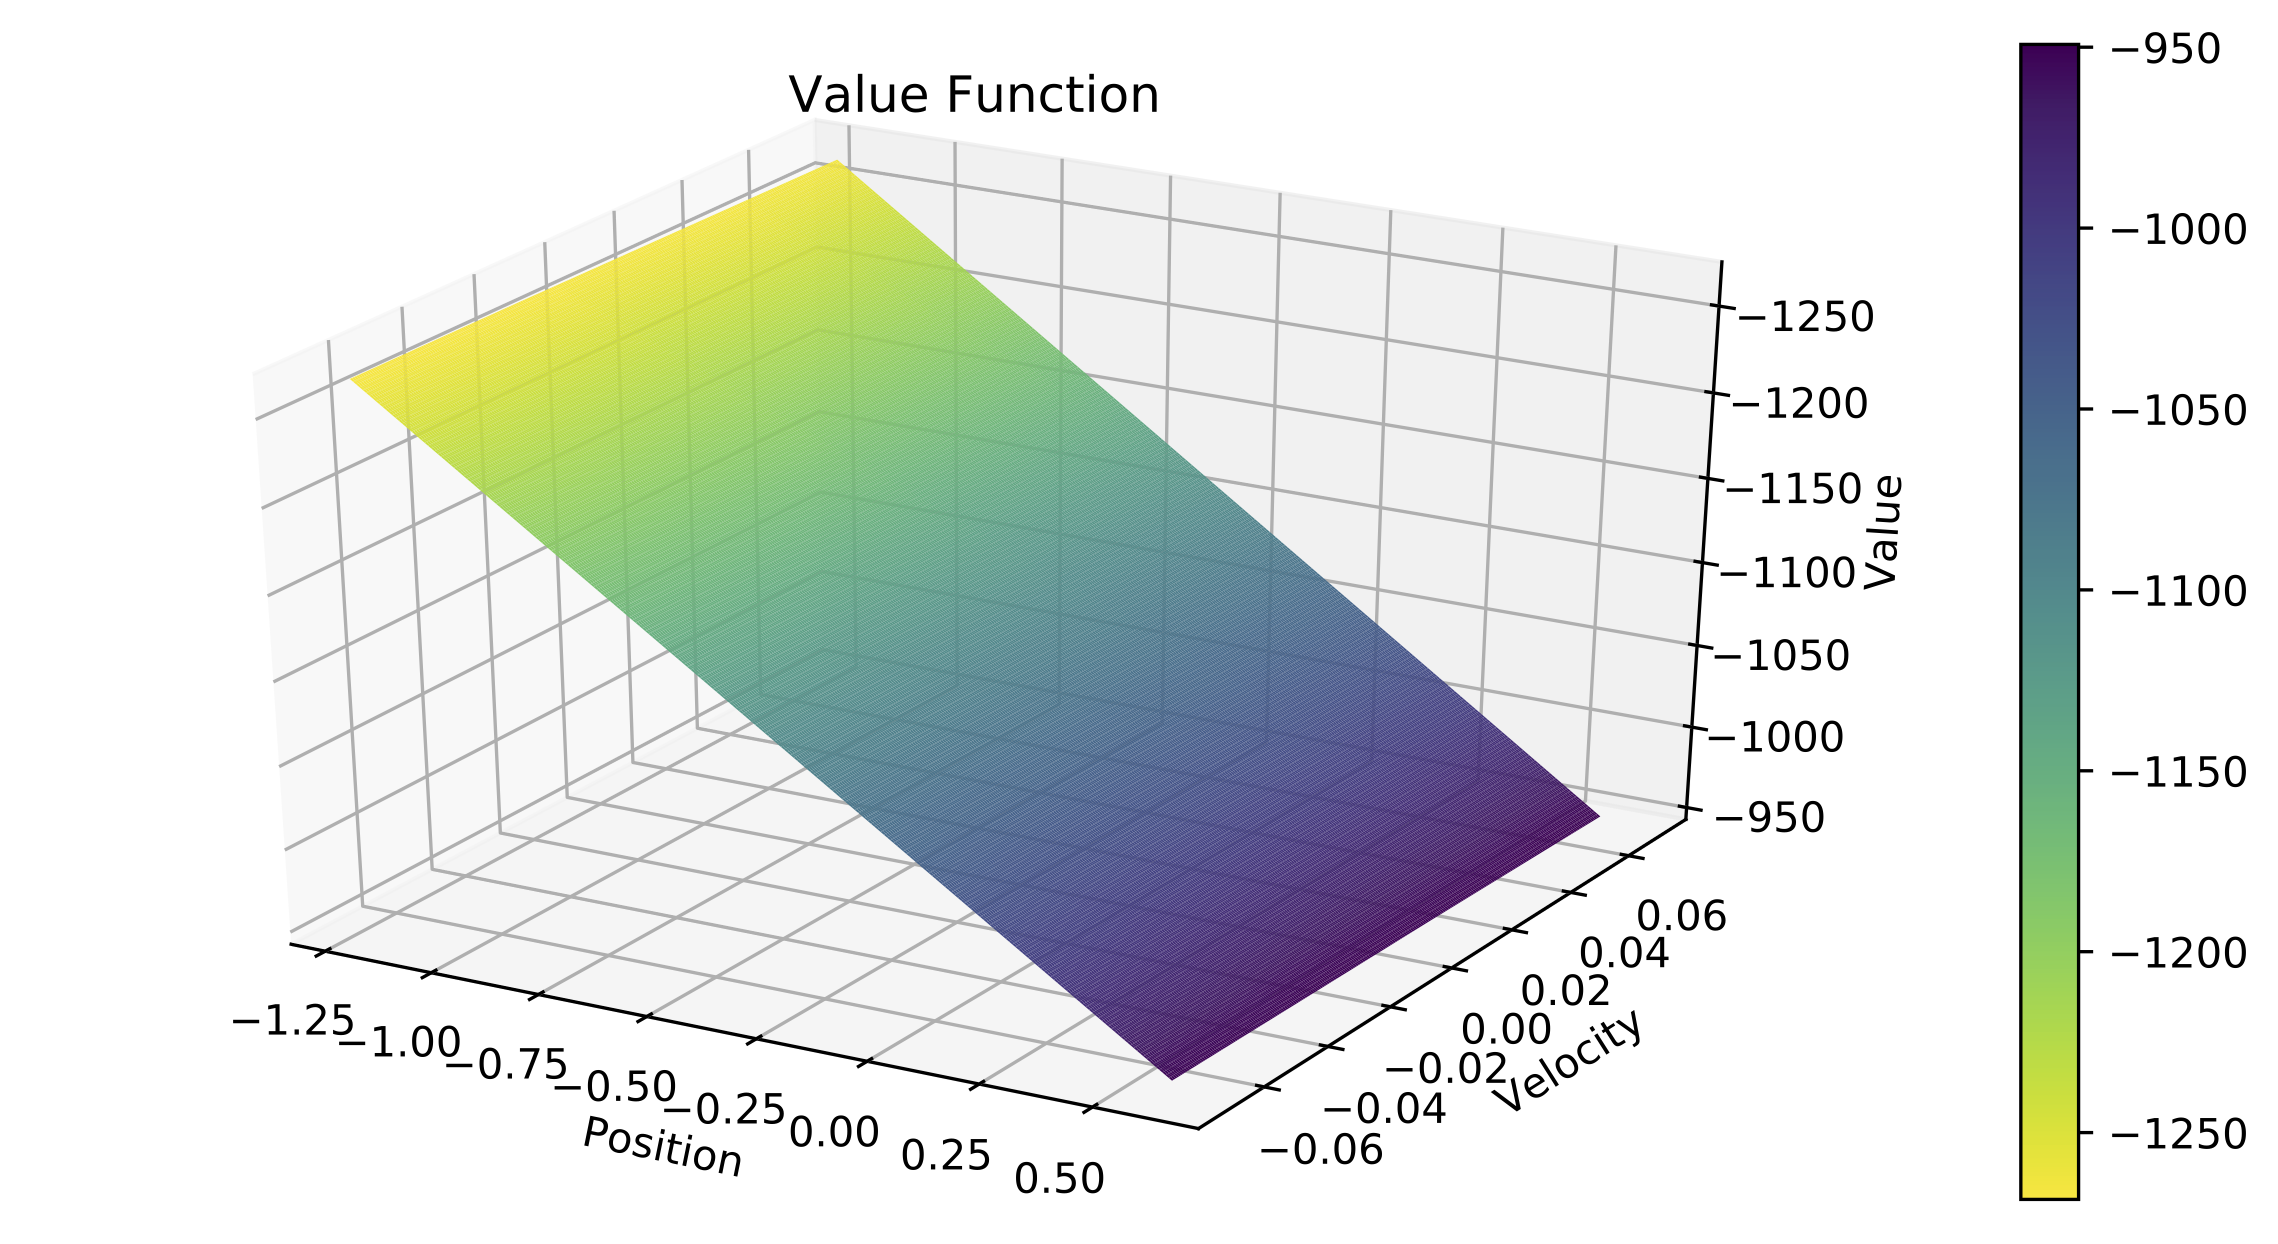
\includegraphics[width=\linewidth]{figs/value_B.png}
        \caption{}
        \label{fig:value_b}
    \end{subfigure}
    \caption{Value function visualizations for both types of features}
    \label{fig:value}
\end{figure}

\begin{enumerate}
\setcounter{enumi}{1}
\item \textbf{[2 points]} For both raw and tile features, we have run Q-learning with some good\footnote{For some sense of good.} parameters and created visualizations of the potential value functions. For each plot in Figure~\ref{fig:value}, write down which features were likely used in Q-learning with function approximation. Explain your reasoning. In addition, interpret each of these plots in the context of the mountain car environment.

\begin{tcolorbox}[fit,height=4cm, width=\linewidth, blank, borderline={1pt}{-2pt},nobeforeafter]
%solution
\end{tcolorbox}


\item \textbf{[2 points]} We see that Figure~\ref{fig:value_b} seems to look like a plane. Can the value function depicted in this plot ever be nonlinear? If so, describe a potential shape. If not explain why. (\textbf{Hint:} How do we calculate the value of a state given the Q-values?)


\begin{tcolorbox}[fit,height=4cm, width=\linewidth, blank, borderline={1pt}{-2pt},nobeforeafter]
%solution
\end{tcolorbox}

    
\end{enumerate}

\begin{figure}[H]
    \centering
    \begin{subfigure}{0.5\textwidth}
        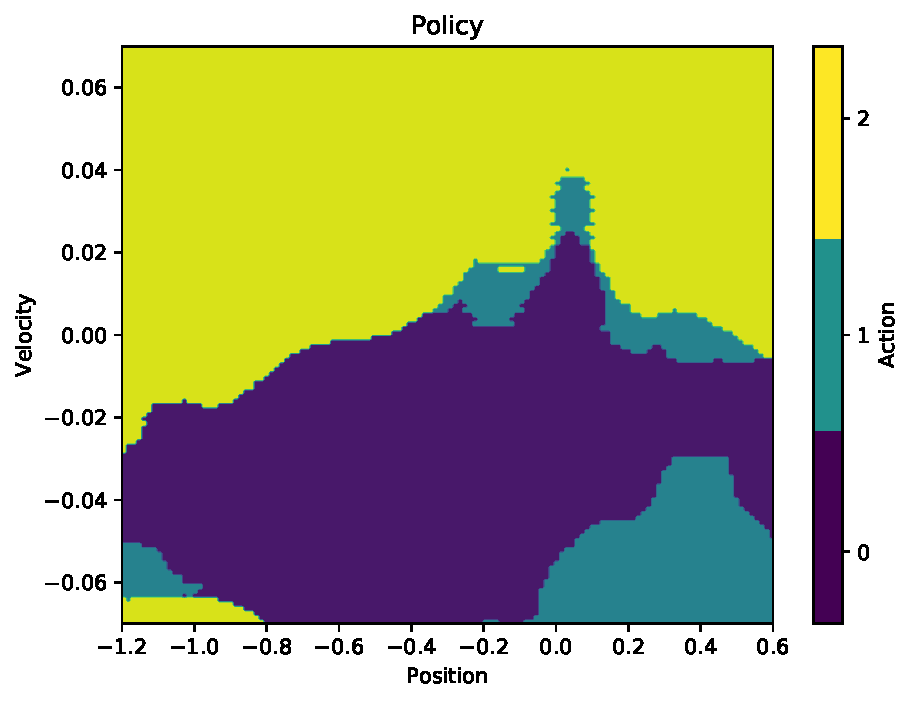
\includegraphics[width=\linewidth]{figs/policy_A.pdf}
        \caption{}
        \label{fig:policy_a}
    \end{subfigure}%
    \begin{subfigure}{0.5\textwidth}
        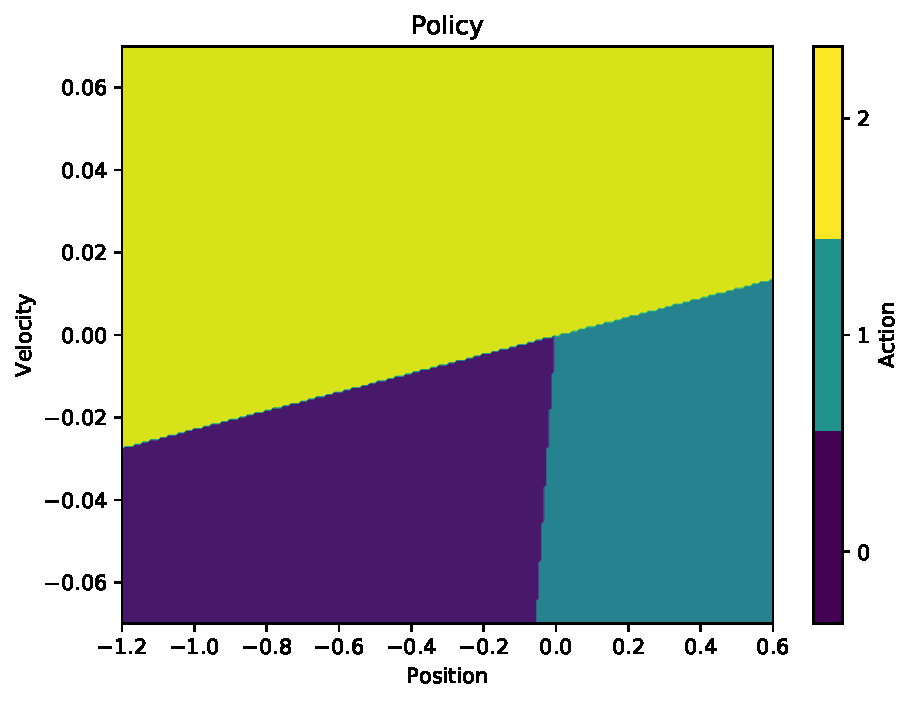
\includegraphics[width=\linewidth]{figs/policy_B.pdf}
        \caption{}
        \label{fig:policy_b}
    \end{subfigure}
    \caption{Policy visualizations for both types of features}
    \label{fig:policy}
\end{figure}


\begin{enumerate}
\setcounter{enumi}{3}
\item \textbf{[2 points]} In a similar fashion to the previous part we have created visualizations of the potential policies learned. For each plot in Figure~\ref{fig:policy} write down which features were likely used in Q-learning with function approximation. Explain your reasoning. In addition, interpret each of these plots in the context of the mountain car environment.
    
\begin{tcolorbox}[fit,height=4cm, width=\linewidth, blank, borderline={1pt}{-2pt},nobeforeafter]
%solution
\end{tcolorbox}

\end{enumerate}